\section{Analysis}
\label{sec:analysis}

\subsection{When does search pay off?}
Synthesizing RQ1--RQ4 yields a simple decision rule for test-time search on this
structured-output task:
\begin{enumerate}
\item \textbf{Search the reasoning, not the taxonomy --- for weak-to-mid
policies.} $\mctsreas$ beats $\mctstax$ on four of five policies
(Table~\ref{tab:m4m5}), and on the weak policy even at \emph{half} the budget
(Figure~\ref{fig:budget}); committing to coarse categories early is the single
most costly design choice. On the premium policy the two are within noise of
each other and of greedy.
\item \textbf{Spend on search when the policy is weak.} The marginal gain over
greedy is large for a weak policy and shrinks toward zero as policy strength
$\polacc$ grows (RQ2); on a strong policy near the task's accuracy ceiling,
additional search is barely worth its cost.
\item \textbf{Prefer reward-guided search to sampling.} At matched budget,
self-consistency---which ignores the reward---captures almost none of the gain that
reward-guided MCTS does (RQ1).
\end{enumerate}
The binding constraints are the \emph{search space} and the \emph{policy}, not the
search budget or the reward source.

\subsection{Cascade error: why taxonomy search hurts}
Proposition~\ref{prop:cascade} predicts that level-by-level commitment compounds
early mistakes. The per-example breakdown (weak policy, $5$ seeds $\times$
$n{=}300$, Figure~\ref{fig:cascade}) confirms it: \textbf{$\mctstax$ commits to a
wrong category --- unrecoverable by construction --- on $60.5\%$ of examples,
versus $51.9\%$ for $\mctsreas$} (greedy: $71.3\%$), and on the examples where
$\mctstax$ chose the wrong category, $\mctsreas$ recovered the correct one
$25.7\%$ of the time. Notably, the within-category error rate (right category,
wrong leaf) is nearly constant across strategies ($14$--$17\%$): all of the
reasoning-search advantage comes from avoiding the early, coarse commitment, not
from finer leaf discrimination. Deferring commitment is thus the mechanism behind
reasoning search's advantage.

\begin{figure}[t]
\centering
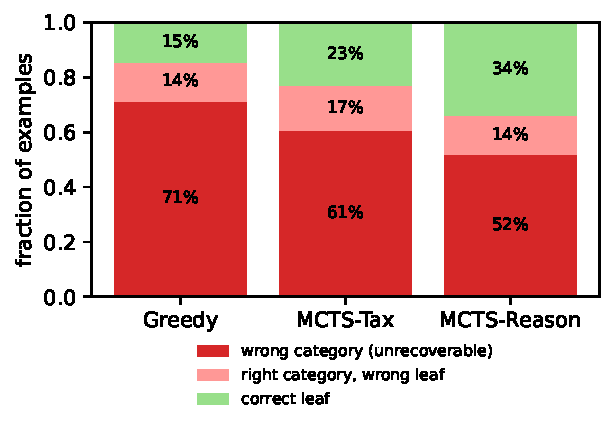
\includegraphics[width=0.8\linewidth]{figures/cascade.pdf}
\caption{First-error level (GPT-4.1-nano, $5$ seeds $\times$ $300$ examples;
greedy is deterministic, $1$ seed). Strategies differ almost entirely in how
often they commit to a wrong coarse category; the right-category-wrong-leaf band
is nearly constant.}
\label{fig:cascade}
\end{figure}

\subsection{The scaffold, not the search}
The $\mctsreas$ budget sweep (Figure~\ref{fig:budget}) adds a sharper reading of
RQ4: accuracy at $I{=}2$ --- where the ``tree'' has barely expanded beyond its
root and the reward has had no opportunity to steer --- already matches $I{=}8$.
Most of the benefit of ``MCTS over reasoning'' is therefore attributable to its
\emph{scaffold} (generate free-form reasoning about the patch, then commit to a
leaf directly, skipping level-by-level commitment), not to the tree-search
machinery on top. This refines the headline: the search-space design dominates
both the budget \emph{and the amount of search itself}. By contrast, $\mctstax$
does benefit from iterations at small $I$ (Figure~\ref{fig:budget}), but
saturates by $I{\approx}8$ at a level far below the reasoning scaffold. The
scaffold reading also explains the premium-policy reversal (RQ4): externalized
step-by-step reasoning is a crutch the strongest policy no longer needs, so what
remains useful there is only the taxonomy's fine-grained discrimination.

\subsection{Reward fidelity is not the bottleneck}
Replacing self-evaluation with a stronger external judge (Claude-Haiku-4.5
judging GPT-4.1-nano) leaves taxonomy search exactly where it was ($22.8$ vs.\
$22.9$ leaf) and lifts reasoning search by $+1.5$ points at $+27\%$ tokens ---
less than the same tokens buy via the search-space choice itself (RQ3). The
asymmetry is informative: in $\mctstax$ the reward only re-ranks siblings
\emph{after} the category commitment that drives most errors
(Figure~\ref{fig:cascade}), so no reward source can rescue it; in $\mctsreas$
the reward selects among complete leaf commitments, where a better judge has
something to act on --- yet the effect is marginal because the policy's own
self-evaluation already separates its candidate commitments about as well.

The logged rollout rewards quantify this directly. Treating the reward of each
MCTS rollout as a predictor of whether that rollout's leaf is correct: on
taxonomy rollouts the judge is \emph{measurably better calibrated} than
self-evaluation (AUROC $0.76$ vs.\ $0.71$, $14$--$24$k pooled rollouts) --- and
final accuracy still does not move, confirming that reward quality is not what
limits $\mctstax$. On reasoning rollouts the judge is \emph{no} better
calibrated ($0.62$ vs.\ $0.64$), consistent with its marginal accuracy effect
there. In both cases the reward ranks candidates far above chance, so the
search is reward-guided in a meaningful sense; it is the set of candidates the
search space exposes, not their ranking, that binds.

\subsection{Latency and practical cost}
Token budget understates MCTS's practical cost, and the right structural
measure is \emph{sequential depth}: the number of LLM rounds that cannot be
parallelized. On our two-level tree, greedy and self-consistency have depth $2$
(samples are independent), best-of-$N$ depth $3$, and beam depth equal to the
number of levels; MCTS iterations, by contrast, are inherently sequential
because each depends on the previous tree statistics --- roughly $2I$ rounds
for $\mctstax$ ($\approx\!34$ at $I{=}16$) and $3I$ for $\mctsreas$
($\approx\!24$ at $I{=}8$, $\approx\!7$ at $I{=}2$). Uncached pilot runs are
consistent: with 10-way example parallelism, Haiku spends $\approx\!47$\,s and
$\approx\!32$\,s of wall clock per example on $\mctstax(16)$ and
$\mctsreas(8)$ respectively, versus seconds for the depth-2 strategies. The
flat $\mctsreas$ iteration curve (Figure~\ref{fig:budget}) is therefore also a
latency result: at $I{=}2$ the best strategy runs at near-interactive depth,
whereas matching $\mctstax$'s budget costs an order of magnitude more
sequential rounds for less accuracy.

\subsection{Failure modes}
We decompose the errors of $\mctstax(16)$ and $\mctsreas(8)$ (weak policy, seed
13, $n{=}300$) along three mechanically computable axes plus one adjudicated
one. \emph{Level:} both strategies make $78\%$ of their errors at the category
level and $22\%$ at the sibling level --- the strategies differ in \emph{how
many} errors they make (231 vs.\ 198), not where. \emph{Reward misranking:} the
gold leaf appeared among the search's own rollout commitments --- found but not
selected --- in $17\%$ of $\mctstax$ errors and $27\%$ of $\mctsreas$ errors;
this slice is the upper bound on what a better reward could recover, and its
size for $\mctsreas$ explains why the external judge helps only there (RQ3).
\emph{Ambiguous gold:} an LLM adjudicator (Claude-Haiku-4.5, shown the patch
and both labels' definitions) judges the model's label a \emph{defensible
alternative} for $42\%$ of sampled $\mctsreas$ errors but only $12\%$ of
$\mctstax$ errors ($50$ samples each). Reasoning search's residual errors are
thus to a large degree single-label artifacts on genuinely multi-label
examples, whereas taxonomy search's errors are mostly outright misses ---
its effective accuracy gap is wider than the headline numbers suggest.

\subsection{Limitations}
\label{sec:limitations}
\begin{itemize}
\item \textbf{Label noise and ambiguity.} BigVul CWE labels are known to be noisy,
and many functions admit several valid CWEs while the gold label is single; this
caps achievable accuracy independently of method (greedy category accuracy plateaus
near $0.40$ even for a premium model on raw functions).
\item \textbf{Scale.} Comparisons use $n{=}300$ ($5$ seeds) for the weak policy
and $n{=}120$--$150$ ($1$--$3$ seeds) for the others, all drawn from one fixed
example file (the smaller sets are prefixes of the larger), with a few per-cell
API failures dropped. The headline effects are large relative to this scale
(across-seed std $\le 1.1$ points; Bonferroni-corrected significance in
Appendix~\ref{app:extra}), but the premium-policy cells in particular would
benefit from more data.
\item \textbf{Saturation of $\mctstax$.} We compare $\mctstax$ up to $I{=}16$
($10.7$k tokens); deeper probes ($I$ up to $128$, full-depth tree, $n{=}8$)
showed predictions frozen well before $I{=}16$, and $\mctsreas$ at \emph{half}
$\mctstax$'s budget already dominates
(Figure~\ref{fig:budget}), so larger taxonomy-search budgets are unlikely to
change the conclusion.
\item \textbf{Reward is zero-shot only.} A trained process reward model could shift
the RQ3 conclusion; we leave it to future work.
\item \textbf{Pretraining exposure.} We cannot fully rule out that LLMs saw test
CVEs during pretraining; a post-cutoff slice is a planned robustness check.
\item \textbf{Granularity coverage.} Findings are established on a 26-CWE
subset of View-1003 (the labels occurring in the data) plus a floor probe at
View-1000; the intermediate regime --- the full 130-CWE View-1003 as used by
NVD --- is the natural target for future work.
\item \textbf{Language coverage.} Data is C/C++-dominated.
\end{itemize}

\subsection{Tree granularity as a boundary condition}
\label{sec:granularity}
Does the picture survive at the full Research-Concepts granularity (View-1000,
$716$ leaves)? A probe ($n{=}50$) says the question itself dissolves there: the
\emph{strongest} policies drop to near-floor --- Sonnet greedy reaches $20\%$
pillar accuracy (10 pillars) and its predicted path passes through the gold node
on only $6\%$ of examples; $\mctstax$ ($I{=}16$), now spending $30$k
tokens/example, lifts this to $28\%$ / $14\%$. Search still moves the needle
(gold-on-path doubles), but from a base so low that no test-time budget makes
the output usable. This is the boundary condition our policy-strength story
predicts: search converts headroom into accuracy only when the policy is above
the floor of the label space (RQ2), and at research granularity it is not ---
which is also why MITRE directs practical CVE mapping to the smaller View-1003
(\S\ref{sec:problem}). Test-time search is a lever \emph{within} the
operational regime, not a way to buy back a label space the policy cannot see.

\subsection{Temporal robustness}
Splitting the $300$ pilot examples by CVE year (2006--16: $n{=}168$; 2017--19:
$n{=}132$) preserves the full strategy ordering in both periods
(weak policy, leaf accuracy, $5$ seeds): greedy $11.3$/$18.9$,
self-consistency $12.4$/$21.8$, $\mctstax$ $16.0$/$31.8$, $\mctsreas$
$33.2$/$35.6$ (old/recent). All strategies score higher on recent CVEs --- a
drift we cannot attribute (different project mix, or greater pretraining
exposure to recent CVEs) --- but the conclusions rest on \emph{within-period}
orderings, which are stable; notably $\mctsreas$ is the least sensitive to the
period ($+2.4$ points old$\to$recent vs.\ $+15.8$ for $\mctstax$).